\documentclass[unknownkeysallowed]{beamer}
\usepackage[french,english]{babel}
\usepackage{../../sty/beamer_js}
\usepackage{../../sty/shortcuts_js}

\addbibresource{../../bib/references_all.bib}

\begin{document}

%%%%%%%%%%%%%%%%%%%%%%%%%%%%%%%%%%%%%%%%%%%%%%%%%%%%%%%%%%%%%%%%%%%%%%%%%%%%%%%
%%%%%%%%%%%%%%%%%%%%%%             Headers               %%%%%%%%%%%%%%%%%%%%%%
%%%%%%%%%%%%%%%%%%%%%%%%%%%%%%%%%%%%%%%%%%%%%%%%%%%%%%%%%%%%%%%%%%%%%%%%%%%%%%%


%%%%%%%%%%%%%%%%%%%%%%%%%%%%%%%%%%%%%%%%%%%%%%%%%%%%%%%%%%%%%%%%%%%%%%%%%%%%%%%
\begin{frame}
\bigskip
\bigskip
\begin{center}{
\LARGE\color{marron}
\textbf{HMMA238: Introduction à git}
\textbf{ }\\
\vspace{0.5cm}
}

\color{marron}
\textbf{}
\end{center}

\begin{center}
\textbf{Joseph Salmon} \\
\vspace{0.1cm}
\url{http://josephsalmon.eu}\\
\vspace{0.5cm}
Université de Montpellier \\
\end{center}

\centering
\includegraphics[width=0.13\textwidth]{umonpellier_logo}

\end{frame}
%%%%%%%%%%%%%%%%%%%%%%%%%%%%%%%%%%%%%%%%%%%%%%%%%%%%%%%%%%%%%%%%%%%%%%%%%%%%%%%




%%%%%%%%%%%%%%%%%%%%%%%%%%%%%%%%%%%%%%%%%%%%%%%%%%%%%%%%%%%%%%%%%%%%%%%%%%%%%%%
%%%%%%%%%%%%%%%%%%%%%%%%       PLAN      %%%%%%%%%%%%%%%%%%%%%%%%%%%%%%%%%%%%%%
%%%%%%%%%%%%%%%%%%%%%%%%%%%%%%%%%%%%%%%%%%%%%%%%%%%%%%%%%%%%%%%%%%%%%%%%%%%%%%%



%%%%%%%%%%%%%%%%%%%%%%%%%%%%%%%%%%%%%%%%%%%%%%%%%%%%%%%%%%%%%%%%%%%%%%%%%%%%%%%
\begin{frame}{Sommaire}
\tableofcontents[hideallsubsections]
\end{frame}
%%%%%%%%%%%%%%%%%%%%%%%%%%%%%%%%%%%%%%%%%%%%%%%%%%%%%%%%%%%%%%%%%%%%%%%%%%%%%%%



%%%%%%%%%%%%%%%%%%%%%%%%%%%%%%%%%%%%%%%%%%%%%%%%%%%%%%%%%%%%%%%%%%%%%%%%%%%%%%%
\AtBeginSection[]
{
\begin{frame}<beamer>{Sommaire}
\tableofcontents[currentsubsection,
    hideothersubsections,
    sectionstyle=show/shaded,
]
\end{frame}
}
%%%%%%%%%%%%%%%%%%%%%%%%%%%%%%%%%%%%%%%%%%%%%%%%%%%%%%%%%%%%%%%%%%%%%%%%%%%%%%%



%%%%%%%%%%%%%%%%%%%%%%%%%%%%%%%%%%%%%%%%%%%%%%%%%%%%%%%%%%%%%%%%%%%%%%%%%%%%%%%
\AtBeginSubsection[]{%
    \begin{frame}<beamer>%
      \frametitle{Sommaire}
      \tableofcontents[currentsection,subsectionstyle=show/shaded/hide]%
    \end{frame}}%
%%%%%%%%%%%%%%%%%%%%%%%%%%%%%%%%%%%%%%%%%%%%%%%%%%%%%%%%%%%%%%%%%%%%%%%%%%%%%%%



%%%%%%%%%%%%%%%%%%%%%%%%%%%%%%%%%%%%%%%%%%%%%%%%%%%%%%%%%%%%%%%%%%%%%%%%%%%%%%%
%%%%%%%%%%%%%%%%%%%%%%%%%%%%%%%%%%%%%%%%%%%%%%%%%%%%%%%%%%%%%%%%%%%%%%%%%%%%%%%
\section{Motivation}
\label{sec:motivation}
%%%%%%%%%%%%%%%%%%%%%%%%%%%%%%%%%%%%%%%%%%%%%%%%%%%%%%%%%%%%%%%%%%%%%%%%%%%%%%%
%%%%%%%%%%%%%%%%%%%%%%%%%%%%%%%%%%%%%%%%%%%%%%%%%%%%%%%%%%%%%%%%%%%%%%%%%%%%%%%


%%%%%%%%%%%%%%%%%%%%%%%%%%%%%%%%%%%%%%%%%%%%%%%%%%%%%%%%%%%%%%%%%%%%%%%%%%%%%%%
\begin{frame}{Crédit:}

\textbf{ Inspiré du travail de Nelle Varoquaux:}

\vspace{3cm}

\url{http://members.cbio.mines-paristech.fr/~nvaroquaux/teaching/2016-aspss/git.html}

\end{frame}
%%%%%%%%%%%%%%%%%%%%%%%%%%%%%%%%%%%%%%%%%%%%%%%%%%%%%%%%%%%%%%%%%%%%%%%%%%%%%%%


%%%%%%%%%%%%%%%%%%%%%%%%%%%%%%%%%%%%%%%%%%%%%%%%%%%%%%%%%%%%%%%%%%%%%%%%%%%%%%%
\begin{frame}{Pourquoi utiliser un gestionnaire de version}


\begin{itemize}
  \item recherche / travail reproductible
  \vspace{1.3cm}

  \item retrouver un ``état'' passé (typiquement un état où tout marchait bien)

  \vspace{1.3cm}

  \item recherche / travail  rapide et efficace (notamment à plusieurs)
\end{itemize}


\end{frame}
%%%%%%%%%%%%%%%%%%%%%%%%%%%%%%%%%%%%%%%%%%%%%%%%%%%%%%%%%%%%%%%%%%%%%%%%%%%%%%%



%%%%%%%%%%%%%%%%%%%%%%%%%%%%%%%%%%%%%%%%%%%%%%%%%%%%%%%%%%%%%%%%%%%%%%%%%%%%%%%
\begin{frame}{Système similaires (limités?)}

\begin{itemize}
  \item dropbox, solutions ``cloud'' et variantes

  \vspace{1.3cm}

  \item Sharelatex (bon en fait on peut l'utiliser avec git aussi)
\end{itemize}

\end{frame}
%%%%%%%%%%%%%%%%%%%%%%%%%%%%%%%%%%%%%%%%%%%%%%%%%%%%%%%%%%%%%%%%%%%%%%%%%%%%%%%




%%%%%%%%%%%%%%%%%%%%%%%%%%%%%%%%%%%%%%%%%%%%%%%%%%%%%%%%%%%%%%%%%%%%%%%%%%%%%%%
\begin{frame}{}
  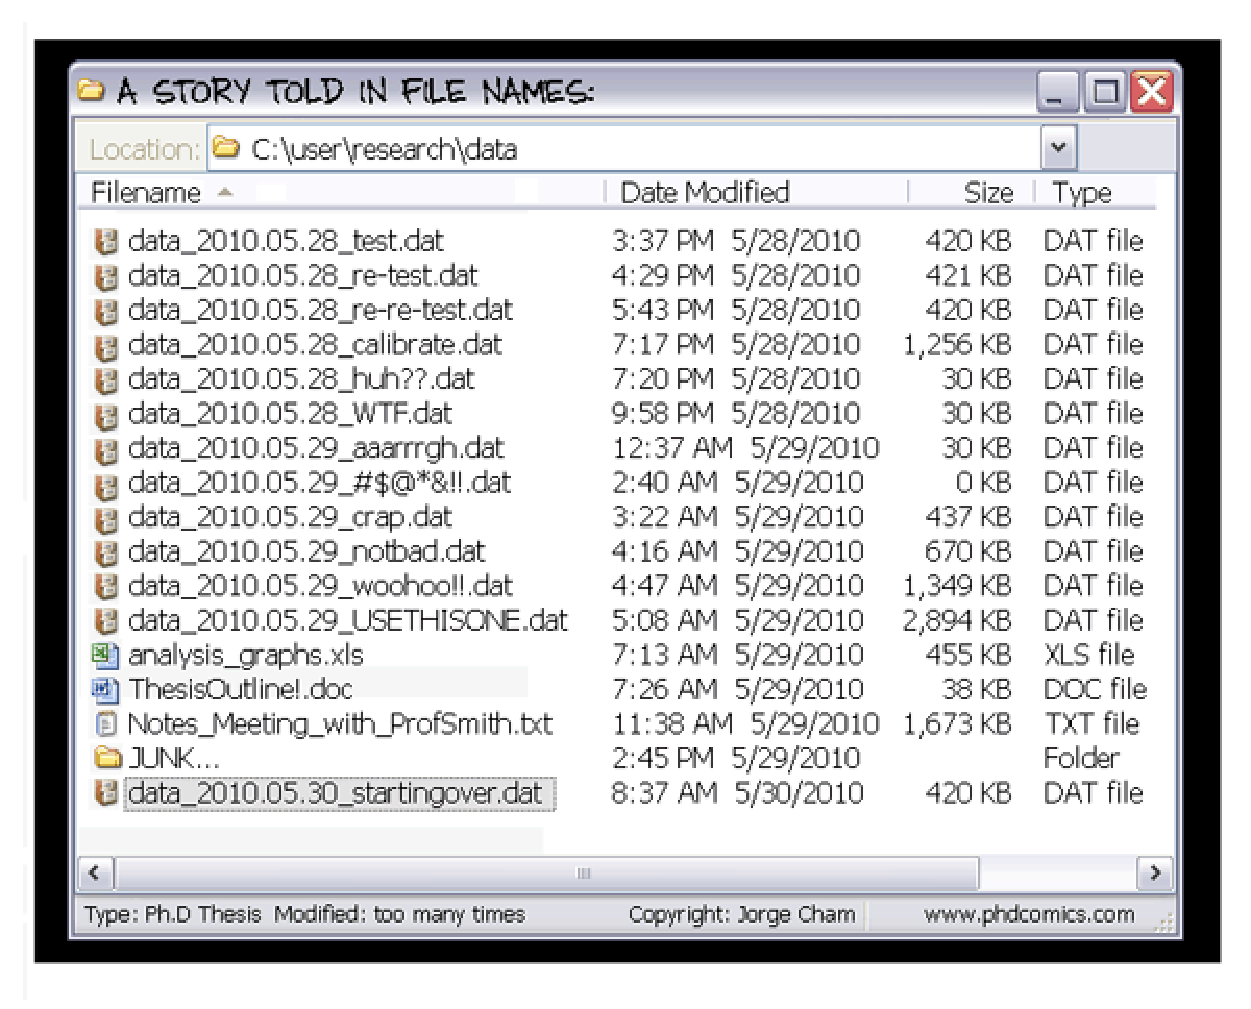
\includegraphics[width=.97\linewidth]{phd052810s}

{\small Credit: "Piled Higher and Deeper" by Jorge Cham: \url{www.phdcomics.com}
}
\end{frame}
%%%%%%%%%%%%%%%%%%%%%%%%%%%%%%%%%%%%%%%%%%%%%%%%%%%%%%%%%%%%%%%%%%%%%%%%%%%%%%%


%%%%%%%%%%%%%%%%%%%%%%%%%%%%%%%%%%%%%%%%%%%%%%%%%%%%%%%%%%%%%%%%%%%%%%%%%%%%%%%
\begin{frame}{Contrôle de version}

\begin{itemize}
  \item garde \underline{\emph{\textbf{TOUT}}} l'historique des versions pour un traçage facile

  \vspace{1.3cm}

  \item bénéficie au travail d'équipe\footnote{``Je suis une bande de jeune à moi tout seul'' (R. Séchan, 1977) }

  \vspace{1.3cm}

  \item Améliore l'efficacité d'écriture (de code ou de texte)

  \vspace{1.3cm}

  \item Travailler sur plusieurs machines sans problème


\end{itemize}
\end{frame}
%%%%%%%%%%%%%%%%%%%%%%%%%%%%%%%%%%%%%%%%%%%%%%%%%%%%%%%%%%%%%%%%%%%%%%%%%%%%%%%



%%%%%%%%%%%%%%%%%%%%%%%%%%%%%%%%%%%%%%%%%%%%%%%%%%%%%%%%%%%%%%%%%%%%%%%%%%%%%%%
\begin{frame}{Visualisation: exemples avec github}

\begin{itemize}
  \item Un petit projet personnel: \url{https://github.com/josephsalmon/OrganizationFiles}

  \vspace{1.3cm}

  \item Un gros projet: \url{https://github.com/scikit-learn/scikit-learn}


\end{itemize}


\end{frame}
%%%%%%%%%%%%%%%%%%%%%%%%%%%%%%%%%%%%%%%%%%%%%%%%%%%%%%%%%%%%%%%%%%%%%%%%%%%%%%%


%%%%%%%%%%%%%%%%%%%%%%%%%%%%%%%%%%%%%%%%%%%%%%%%%%%%%%%%%%%%%%%%%%%%%%%%%%%%%%%
\begin{frame}{Exercices}

\exo{Commencez par vous créer un compte \texttt{github} si ce n'est pas déjà le cas}

\vspace{1.5cm}
\exo{Vérifier que \texttt{git} est installée sur votre machine, sinon:

(Linux / Ubuntu): \texttt{sudo apt-get install git}

}

\vspace{0.5cm}

\rem \texttt{sudo apt-get install tig } peut-être utile
\end{frame}
%%%%%%%%%%%%%%%%%%%%%%%%%%%%%%%%%%%%%%%%%%%%%%%%%%%%%%%%%%%%%%%%%%%%%%%%%%%%%%%


%%%%%%%%%%%%%%%%%%%%%%%%%%%%%%%%%%%%%%%%%%%%%%%%%%%%%%%%%%%%%%%%%%%%%%%%%%%%%%%
%%%%%%%%%%%%%%%%%%%%%%%%%%%%%%%%%%%%%%%%%%%%%%%%%%%%%%%%%%%%%%%%%%%%%%%%%%%%%%%
\section{Démarrer}
\label{sec:démarrer}
%%%%%%%%%%%%%%%%%%%%%%%%%%%%%%%%%%%%%%%%%%%%%%%%%%%%%%%%%%%%%%%%%%%%%%%%%%%%%%%
%%%%%%%%%%%%%%%%%%%%%%%%%%%%%%%%%%%%%%%%%%%%%%%%%%%%%%%%%%%%%%%%%%%%%%%%%%%%%%%


%%%%%%%%%%%%%%%%%%%%%%%%%%%%%%%%%%%%%%%%%%%%%%%%%%%%%%%%%%%%%%%%%%%%%%%%%%%%%%%
\begin{frame}[fragile]{Créer un projet}

\begin{itemize}
  \item Initialisation : nouveau projet
\end{itemize}
\begin{lstlisting}
$ git init
Initialized empty Git repository in /home/jo/Downloads/CES/.git/
\end{lstlisting}

\begin{itemize}
  \item Initialisation : projet existant
\end{itemize}

\begin{lstlisting}
$ git clone git@github.com:josephsalmon/OrganizationFiles.git
\end{lstlisting}

\end{frame}
%%%%%%%%%%%%%%%%%%%%%%%%%%%%%%%%%%%%%%%%%%%%%%%%%%%%%%%%%%%%%%%%%%%%%%%%%%%%%%%



%%%%%%%%%%%%%%%%%%%%%%%%%%%%%%%%%%%%%%%%%%%%%%%%%%%%%%%%%%%%%%%%%%%%%%%%%%%%%%%
\begin{frame}[fragile]{Configurer \texttt{git}}

\begin{itemize}
  \item Localement : seulement le répertoire \texttt{git} courant sera affecté
\end{itemize}
\begin{lstlisting}
$ git config [options]
\end{lstlisting}

\begin{itemize}
  \item Pour l'utilisateur courant : la configuration de l'utilisateur sera modifié dans le fichier \texttt{~/.git/config}
\end{itemize}

\begin{lstlisting}
$ git config --global [options]
\end{lstlisting}


\begin{itemize}
  \item Globally: toues les utilisateurs du système seront affectés
\end{itemize}

\begin{lstlisting}
$ git config --system [options]
\end{lstlisting}


\end{frame}
%%%%%%%%%%%%%%%%%%%%%%%%%%%%%%%%%%%%%%%%%%%%%%%%%%%%%%%%%%%%%%%%%%%%%%%%%%%%%%%





%%%%%%%%%%%%%%%%%%%%%%%%%%%%%%%%%%%%%%%%%%%%%%%%%%%%%%%%%%%%%%%%%%%%%%%%%%%%%%%
\begin{frame}[fragile]{Configurer \texttt{git} (II)}

\begin{itemize}
  \item Identité :
\end{itemize}
\begin{lstlisting}
$ git config --global user.name "Your Name Comes Here"
$ git config --global user.email you@yourdomain.com
\end{lstlisting}

\begin{itemize}
  \item Pour choisir l'éditeur (qui lira les différences)
\end{itemize}

\begin{lstlisting}
$ git config --global core.editor vim\end{lstlisting}

\begin{itemize}
  \item Vérifier son système
\end{itemize}

\begin{lstlisting}
    $ git config --list
\end{lstlisting}


\end{frame}
%%%%%%%%%%%%%%%%%%%%%%%%%%%%%%%%%%%%%%%%%%%%%%%%%%%%%%%%%%%%%%%%%%%%%%%%%%%%%%%



%%%%%%%%%%%%%%%%%%%%%%%%%%%%%%%%%%%%%%%%%%%%%%%%%%%%%%%%%%%%%%%%%%%%%%%%%%%%%%%
\begin{frame}[fragile]{Commandes fondamentales}

\begin{itemize}
  \item \lstinline[basicstyle =\ttfamily]+git add+: ajoute un fichier à la ``capture'' souhaitée
\end{itemize}
\begin{lstlisting}
$ git add README
\end{lstlisting}

\begin{itemize}
  \item \lstinline[basicstyle =\ttfamily]+git commit+: sauvegarde tous les fichiers ajouter dans la capture:
\end{itemize}

\begin{lstlisting}
$ git commit -m "Mon message de commit"
\end{lstlisting}
\begin{itemize}
  \item \lstinline[basicstyle =\ttfamily]+git status+: montre le statut des fichiers du dépôt
  \item \lstinline[basicstyle =\ttfamily]+git log+: montre les logs des commits
\end{itemize}
\end{frame}
%%%%%%%%%%%%%%%%%%%%%%%%%%%%%%%%%%%%%%%%%%%%%%%%%%%%%%%%%%%%%%%%%%%%%%%%%%%%%%%




%%%%%%%%%%%%%%%%%%%%%%%%%%%%%%%%%%%%%%%%%%%%%%%%%%%%%%%%%%%%%%%%%%%%%%%%%%%%%%%
\begin{frame}{Status des fichiers}

\begin{itemize}
  \item fichiers tracés \english{tracked files}
  \begin{itemize}
    \vspace{0.7cm}

    \item non modifié \english{unmodified}
    \vspace{0.7cm}

    \item modifié \english{modified}
    \vspace{0.7cm}

    \item organisé \english{staged}
  \end{itemize}

\vspace{1.3cm}

  \item fichiers non tracés \english{untracked files}: tout le reste

\end{itemize}

\end{frame}
%%%%%%%%%%%%%%%%%%%%%%%%%%%%%%%%%%%%%%%%%%%%%%%%%%%%%%%%%%%%%%%%%%%%%%%%%%%%%%%


%%%%%%%%%%%%%%%%%%%%%%%%%%%%%%%%%%%%%%%%%%%%%%%%%%%%%%%%%%%%%%%%%%%%%%%%%%%%%%%
\begin{frame}{Cycle de vie des fichiers versionnés}

\begin{center}

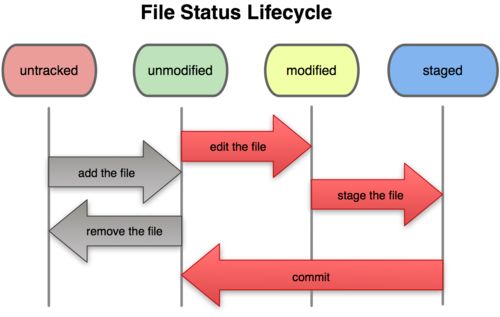
\includegraphics[width=.97\linewidth]{git_file_status_lifecycle}

Crédit: \url{https://git-scm.com/book/en/v2}
\end{center}

\end{frame}
%%%%%%%%%%%%%%%%%%%%%%%%%%%%%%%%%%%%%%%%%%%%%%%%%%%%%%%%%%%%%%%%%%%%%%%%%%%%%%%


%%%%%%%%%%%%%%%%%%%%%%%%%%%%%%%%%%%%%%%%%%%%%%%%%%%%%%%%%%%%%%%%%%%%%%%%%%%%%%%
\begin{frame}{Exercice}

\exo{Faire \lstinline[basicstyle =\ttfamily]+01_configuring_and_committing.rst+ dans
{\tiny\url{http://members.cbio.mines-paristech.fr/~nvaroquaux/teaching/2016-aspss/exercises.zip}}}

\end{frame}
%%%%%%%%%%%%%%%%%%%%%%%%%%%%%%%%%%%%%%%%%%%%%%%%%%%%%%%%%%%%%%%%%%%%%%%%%%%%%%%


%%%%%%%%%%%%%%%%%%%%%%%%%%%%%%%%%%%%%%%%%%%%%%%%%%%%%%%%%%%%%%%%%%%%%%%%%%%%%%%
\begin{frame}[fragile]{Effacer / déplacer des fichier}

% \begin{itemize}
% \item \lstinline[basicstyle =\ttfamily]+git rm+: enlève un fichier de l'arborescence de travail
% \end{itemize}

% \begin{lstlisting}
% $ git rm FILENAME
% \end{lstlisting}

\begin{itemize}
  \item \lstinline[basicstyle =\ttfamily]+git mv+: déplace / renomme un fichier
\end{itemize}

\begin{lstlisting}
$ git mv FILENAME TARGET
\end{lstlisting}

\end{frame}
%%%%%%%%%%%%%%%%%%%%%%%%%%%%%%%%%%%%%%%%%%%%%%%%%%%%%%%%%%%%%%%%%%%%%%%%%%%%%%%


%%%%%%%%%%%%%%%%%%%%%%%%%%%%%%%%%%%%%%%%%%%%%%%%%%%%%%%%%%%%%%%%%%%%%%%%%%%%%%%
\begin{frame}{Branches}


\begin{itemize}
\item \lstinline[basicstyle =\ttfamily]+git branch+: gère les branches

\begin{itemize}
  \item
  \lstinline[basicstyle =\ttfamily]+git branch+: liste les branches du dépôt locale
  \item
  \lstinline[basicstyle =\ttfamily]+git branch [branch_name]+: créer une branche
  \item
  \lstinline[basicstyle =\ttfamily]+git branch -d [branch_name]+: efface une branche
\end{itemize}

\vspace{0.6cm}

\item \lstinline[basicstyle =\ttfamily]+git checkout+: gère les déplacements

\begin{itemize}
  \item \lstinline[basicstyle =\ttfamily]+git checkout [branch_name]+: bouge la branche
  \item \lstinline[basicstyle =\ttfamily]+git checkout -b [branch_name]+: crée et déplace la branche \lstinline[basicstyle =\ttfamily]+branch_name+
\end{itemize}
\end{itemize}

\end{frame}
%%%%%%%%%%%%%%%%%%%%%%%%%%%%%%%%%%%%%%%%%%%%%%%%%%%%%%%%%%%%%%%%%%%%%%%%%%%%%%%



%%%%%%%%%%%%%%%%%%%%%%%%%%%%%%%%%%%%%%%%%%%%%%%%%%%%%%%%%%%%%%%%%%%%%%%%%%%%%%%
\begin{frame}[fragile]{Serveur distant}

Ici github, ou un autre serveur rentre en jeu, typiquement avec la commande:

\vspace{0.5cm}
\begin{lstlisting}
$ git clone git@github.com:josephsalmon/OrganizationFiles.git
\end{lstlisting}

\vspace{0.5cm}


\begin{itemize}
  \item
\lstinline[basicstyle =\ttfamily]+git push [remote-name] [branch-name]+: pousse [branch-name] sur le serveur distant et la branche [branch-name]

\vspace{0.39cm}

  \item
\lstinline[basicstyle =\ttfamily]+git pull [remote-name] [branch-name]:+ tire [branch-name] depuis le serveur distant [branch-name]

\end{itemize}

\end{frame}
%%%%%%%%%%%%%%%%%%%%%%%%%%%%%%%%%%%%%%%%%%%%%%%%%%%%%%%%%%%%%%%%%%%%%%%%%%%%%%%


% %%%%%%%%%%%%%%%%%%%%%%%%%%%%%%%%%%%%%%%%%%%%%%%%%%%%%%%%%%%%%%%%%%%%%%%%%%%%%%%
% \begin{frame}[allowframebreaks]
% \frametitle{Bibliographie}
% \footnotesize
% \printbibliography
% \end{frame}
%  %%%%%%%%%%%%%%%%%%%%%%%%%%%%%%%%%%%%%%%%%%%%%%%%%%%%%%%%%%%%%%%%%%%%%%%%%%%%%%



\end{document}